\documentclass{report}
\usepackage{textcase}
\usepackage{amsmath}
\usepackage{amsfonts}
\usepackage{amssymb}
\usepackage[utf8]{vietnam}
\usepackage{graphicx}
\usepackage{scrextend}
\usepackage[left=3.5cm,right=2cm,top=3.5cm,bottom=3cm]{geometry}
\usepackage{xhfill}
\usepackage{floatrow}
\usepackage{subfigure}
\usepackage{wrapfig}
\usepackage{lipsum}
\usepackage{lettrine}
\usepackage[
    backend=biber,
    style=authoryear,
    natbib=true,
    url=true, 
    doi=true,
    eprint=false
]{biblatex}
\usepackage{hyperref}
\hypersetup{
	colorlinks=false,
	linkcolor=blue,
	filecolor=magenta,      
	urlcolor=cyan,
}
\addbibresource{myref.bib}

\begin{document}
\newcommand{\xfill}[2][1ex]{{%
  \dimen0=#2\advance\dimen0 by #1
  \leaders\hrule height \dimen0 depth -#1\hfill%
}}

%Page 1
\changefontsizes[14pt]{12pt}
\centerline{TỔNG LIÊN ĐOÀN LAO ĐỘNG VIỆT NAM}

\changefontsizes[14pt]{11pt}
\centerline{\textbf{TRƯỜNG ĐẠI HỌC TÔN ĐỨC THẮNG}}
\centerline{\textbf{KHOA CÔNG NGHỆ THÔNG TIN}}

\begin{center}
    \begin{figure}[htp]
    \begin{center}
     
\includegraphics[scale=.2]{logo}
    \end{center}
    \end{figure}
\end{center}

\changefontsizes{16pt}
\centerline{\textbf{BÁO CÁO CUỐI KỲ: KHAI THÁC DỮ LIỆU}}

\centerline{\textbf{VÀ KHAI PHÁ TRI THỨC}}
\vspace{1.5cm}
\changefontsizes{24pt}
\centerline{\textbf{OBJECT RECOGNITION}}

\centerline{\textbf{AND CLASSIFICATION}}

\vspace{3.5cm}
\begin{flushright}
\renewcommand{\baselinestretch}{0.05}
\changefontsizes{14pt}
\textit{Người hướng dẫn: }\textbf{PhD Trần Thanh Phước}
\setlength{\parskip}{0.5em}

\textit{Người thực hiện: }\textbf{Huỳnh Văn Duy - 51703006}

\textbf{Trần Quốc Lĩnh - 51703124}
\setlength{\parskip}{0.5em}


Khoá: \textbf{21}
\setlength{\parskip}{0.5em}

\end{flushright}

\vspace{1.5cm}
\changefontsizes{14pt}
\centerline{\textbf{THÀNH PHỐ HỒ CHÍ MINH, NĂM 2019}}

%Page 2
\newpage
\changefontsizes[14pt]{12pt}
\centerline{TỔNG LIÊN ĐOÀN LAO ĐỘNG VIỆT NAM}

\changefontsizes[14pt]{11pt}
\centerline{\textbf{TRƯỜNG ĐẠI HỌC TÔN ĐỨC THẮNG}}
\centerline{\textbf{KHOA CÔNG NGHỆ THÔNG TIN}}

\begin{center}
	\begin{figure}[htp]
		\begin{center}
			
\includegraphics[scale=.2]{logo}
		\end{center}
	\end{figure}
\end{center}

\changefontsizes{16pt}
\centerline{\textbf{BÁO CÁO CUỐI KỲ: KHAI THÁC DỮ LIỆU}}

\centerline{\textbf{VÀ KHAI PHÁ TRI THỨC}}
\vspace{1.5cm}
\changefontsizes{24pt}
\centerline{\textbf{OBJECT RECOGNITION}}

\centerline{\textbf{AND CLASSIFICATION}}

\vspace{3.5cm}
\begin{flushright}
	\renewcommand{\baselinestretch}{0.05}
	\changefontsizes{14pt}
	\textit{Người hướng dẫn: }\textbf{PhD Trần Thanh Phước}
	\setlength{\parskip}{0.5em}
	
	\textit{Người thực hiện: }\textbf{Huỳnh Văn Duy - 51703006}
	
	\textbf{Trần Quốc Lĩnh - 51703124}
	\setlength{\parskip}{0.5em}
	
	
	Khoá: \textbf{21}
	\setlength{\parskip}{0.5em}
	
\end{flushright}

\vspace{1.5cm}
\changefontsizes{14pt}
\centerline{\textbf{THÀNH PHỐ HỒ CHÍ MINH, NĂM 2019}}



% Page 3
\newpage
\changefontsizes{16pt}
\centerline{\textbf{LỜI CẢM ƠN}}

\changefontsizes{13pt}
\bigskip
\setlength{\parindent}{2cm}


Cảm ơn thầy Trần Thanh Phước đã dạy môn Khai thác dữ liệu và khai phá tri thức hết sức nhiệt tình và tâm huyết, cảm ơn thầy đã định hướng và tạo cơ sở đểnchúng em có thể tự tìm hiểu và học thêm về ...

Còn đây là đồ án của chúng em, sản phẩm của quá trình học tập và rèn luyện dưới sự chỉ dẫn của thầy. Trong quá trình làm bài đồ án này, chúng em vẫn còn nhiều thiếu sót. Chúng em rất mong nhận được sự đánh giá và chỉ bảo từ thầy!
    
% Page 4
\newpage
\changefontsizes{16pt}
\centerline{\textbf{BÀI TẬP LỚN ĐƯỢC HOÀN THÀNH}}
\centerline{\textbf{TẠI TRƯỜNG ĐẠI HỌC TÔN ĐỨC THẮNG}}
\changefontsizes{13pt}
\vspace{1cm}
\setlength{\parindent}{2cm}
Chúng em xin cam đoan đây là sản phẩm bài tập lớn của riêng chúng em. Các nội dung nghiên cứu, kết quả trong đề tài này là trung thực và chưa công bố dưới bất kỳ hình thức nào trước đây. Những số liệu ,hình ảnh được chính chúng em thu thập từ các nguồn khác nhau có ghi rõ trong phần tài liệu tham khảo.

\setlength{\parindent}{2cm}
Ngoài ra, trong bài tiểu luận còn sử dụng một số nhận xét, đánh giá cũng như số liệu của các tác giả khác, cơ quan tổ chức khác đều có trích dẫn và chú thích nguồn gốc.

\setlength{\parindent}{2cm}
Nếu phát hiện có bất kỳ sự gian lận nào chúng em xin hoàn toàn chịu trách nhiệm về nội dung bài tập lớn của mình. Trường đại học Tôn Đức Thắng không liên quan đến những vi phạm tác quyền, bản quyền do chúng em gây ra trong quá trình thực hiện (nếu có).

\vspace{0.75cm}
\begin{flushright}
\renewcommand{\baselinestretch}{0.05}
\changefontsizes{13pt}
\textit{TP. Hồ Chí Minh, ngày 13 tháng 11 năm 2019}
\end{flushright}

\setlength{\parindent}{12.5cm}
\textit{Tác giả 1}\\

\setlength{\parindent}{12.5cm}
\textit{(Đã ký)}\\

\setlength{\parindent}{12cm}
\textit{Huỳnh Văn Duy}\\


\setlength{\parindent}{12.5cm}
\textit{Tác giả 2}\\

\setlength{\parindent}{12.5cm}
\textit{(Đã ký)}\\

\setlength{\parindent}{12cm}
\textit{Trần Quốc Lĩnh}\\


% Page 5
\newpage
\changefontsizes{16pt}
\centerline{\textbf{PHẦN XÁC NHẬN VÀ ĐÁNH GIÁ CỦA GIẢNG VIÊN}}
\bigskip
\changefontsizes{13pt}
\setlength{\parindent}{2.2cm}
Phần xác nhận của GV hướng dẫn

\vspace{0.8cm}
\setlength{\parindent}{1cm}
\ \xfill{1pt} \

\bigskip
\ \xfill{1pt} \

\bigskip
\ \xfill{1pt} \

\bigskip
\ \xfill{1pt} \

\bigskip
\ \xfill{1pt} \

\bigskip
\ \xfill{1pt} \

\changefontsizes{12pt}
\setlength{\parindent}{8cm}
Tp. Hồ Chí Minh, ngày 13 tháng 11 năm 2019

\setlength{\parindent}{11cm}
\textit{(kí và ghi họ tên)}

\changefontsizes{13pt}
\vspace{2.5cm}
\setlength{\parindent}{2.2cm}
Phần đánh giá của GV chấm bài

\vspace{0.8cm}
\setlength{\parindent}{1cm}
\ \xfill{1pt} \

\bigskip
\ \xfill{1pt} \

\bigskip
\ \xfill{1pt} \

\bigskip
\ \xfill{1pt} \

\bigskip
\ \xfill{1pt} \

\bigskip
\ \xfill{1pt} \

\changefontsizes{12pt}
\setlength{\parindent}{8cm}
Tp. Hồ Chí Minh, ngày 13 tháng 11 năm 2019

\setlength{\parindent}{11cm}
\textit{(kí và ghi họ tên)}

% Page 6
\newpage
\changefontsizes{16pt}
\centerline{\textbf{TÓM TẮT}}\

\changefontsizes{13pt}
\setlength{\parindent}{2cm}
Nhằm tổng kết lại toàn bộ kiến thức đã được học và vận dụng vào một bài toán thực tế, nhóm xin thực hiện bài tập cuối kỳ với đề tài: Nhận diện sinh viên trường Đại học Tôn Đức Thắng và đánh giá sinh viên có đang mặc trang trang phục đúng quy định hay không.

Phần trình bày của báo cáo này bao gồm các nội dung chính:

\setlength{\parindent}{2.5cm}
- Tìm hiểu và thu thập dữ liệu

- Mô tả giải thuật

- Kết quả

- Tổng kết

%Page 7
\newpage
\changefontsizes{16pt}
\centerline{\textbf{MỤC LỤC}}\

\vspace{1.2cm}
\changefontsizes{14pt}
\setlength{\parindent}{0cm}
\hyperlink{page.3}{LỜI CẢM ƠN\dotfill\ 3}

\smallskip
\hyperlink{page.4}{CAM KẾT\dotfill\ 4}

\smallskip
\hyperlink{page.5}{ĐÁNH GIÁ CỦA GIÁO VIÊN\dotfill\ 5}

\smallskip
\hyperlink{page.6}{TÓM TẮT\dotfill\ 6}

\smallskip
\hyperlink{page.7}{MỤC LỤC\dotfill\ 7}

\smallskip
\hyperlink{page.8}{DANH MỤC CHÚ THÍCH CÁC HÌNH ẢNH\dotfill\ 8}

\smallskip
\setlength{\parindent}{0.0cm}
\hyperlink{page.9}{CHƯƠNG 1: TÌM HIỂU VÀ THU THẬP DỮ LIỆU\dotfill\ 9}

\setlength{\parindent}{0.5cm}
\hyperlink{page.9}{1.1 Tổng quan về phương pháp giải quyết\dotfill\ 9}

\hyperlink{page.9}{1.2 Thu thập dữ liệu\dotfill\ 9}

\setlength{\parindent}{1cm}
\hyperlink{page.9}{1.2.1. Cách thức thu thập dữ liệu\dotfill\ 9}

\hyperlink{page.10}{1.2.2. Xử lý dữ liệu đầu\dotfill\ 10}



\smallskip
\setlength{\parindent}{0.0cm}
\hyperlink{page.11}{CHƯƠNG 2: GIẢI THUẬT\dotfill\ 11}

\setlength{\parindent}{0.5cm}

\hyperlink{page.11}{2.1. Thế nào là Object recognition và Classification?\dotfill\ 11}

	
\hyperlink{page.11}{2.2. YOLO\dotfill\ 11}


\hyperlink{page.14}{2.3. YOLOv3\dotfill\ 14}


\smallskip
\setlength{\parindent}{0.0cm}
\hyperlink{page.15}{CHƯƠNG 3: KẾT QUẢ\dotfill\ 15}

\setlength{\parindent}{0.5cm}
\hyperlink{page.15}{3.1. Kết quả thực nghiệm\dotfill\ 15}

\setlength{\parindent}{0.5cm}
\hyperlink{page.16}{3.2. Đánh giá kết quả\dotfill\ 16}

\smallskip
\setlength{\parindent}{0.0cm}
\hyperlink{page.17}{CHƯƠNG 4: TỔNG KẾT\dotfill\ 17}

\setlength{\parindent}{0.5cm}
\hyperlink{page.17}{4.1 Thành quả đạt được\dotfill\ 17}

\hyperlink{page.17}{4.2. Hạn chế\dotfill\ 17}

\hyperlink{page.17}{4.3. Hướng mở rộng\dotfill\ 17}

\setlength{\parindent}{0cm}
\smallskip
\hyperlink{page.18}{TÀI LIỆU THAM KHẢO\dotfill\ 18}


%Page 8
\newpage
\changefontsizes{16pt}
\centerline{\textbf{DANH MỤC CHÚ THÍCH CÁC HÌNH ẢNH}}

\vspace{1cm}
\changefontsizes{14pt}
\setlength{\parindent}{0cm}
\bigskip
\textbf{Hình ảnh}

\smallskip
\setlength{\parindent}{1cm}
\changefontsizes{13pt}
\hyperlink{page.9}{Hình 1: Một phần của tập dữ liệu thu thập được}

\smallskip
\hyperlink{page.10}{Hình 2: Đóng khung và gắn label cho ảnh}

\smallskip
\hyperlink{page.12}{Hình 3: Luồng công việc của model YOLO}

\smallskip
\hyperlink{page.12}{Hình 4: Kiến trúc mạng (Network Architecture) của YOLO}

\smallskip
\hyperlink{page.13}{Hình 5: $B$ khung xung quanh ô $i$}


\smallskip
\hyperlink{page.15}{Hình 6: Kết quả thực nghiệm}


%Page ??
\newpage
\changefontsizes{16pt}
\centerline{\textbf{\hyperlink{page.7}{CHƯƠNG 1: TÌM HIỂU VÀ THU THẬP DỮ LIỆU}}}



\bigskip
\changefontsizes{14pt}
\setlength{\parindent}{0.0cm}
\textbf{1.1 Tổng quan về phương pháp giải quyết.}

\smallskip
\changefontsizes{13pt}
\setlength{\parindent}{1cm}
Với đề tài \textit{Nhận diện sinh viên trường Đại học Tôn Đức Thắng và đánh giá sinh viên có đang mặc trang phục đúng quy định hay không}, chúng ta dễ dàng nhận thấy được có hai tác vụ chính cần xử lý đó là: \textit{Nhận diện} và \textit{Đánh giá}.

Đầu tiên, cũng như là phần quan trọng nhất trong tất cả các bài toán về xử lý dữ liệu, đó là thu thập và xử lý dữ liệu như thế nào. Còn về phương pháp, giải thuật sử dụng cho việc nhận diện và đánh giá sẽ được trình bày cụ thể ở chương 2. 

\leftskip0cm
\bigskip
\changefontsizes{14pt}
\setlength{\parindent}{0.0cm}
\textbf{1.2 Thu thập dữ liệu.}


\smallskip
\changefontsizes{13pt}
\setlength{\parindent}{1cm}
Để tăng tính chính xác và thực tế, toàn bộ dữ liệu (ảnh) đều được thu thập tại trường Đại học Tôn Đức Thắng. Tuy nhiên do còn nhiều hạn chế nên tổng số dữ liệu  chỉ khoảng 150 mẫu (ảnh).

\bigskip
\changefontsizes{14pt}
\setlength{\parindent}{0.5cm}
\textbf{1.2.1. Cách thức thu thập dữ liệu.}

\leftskip0.5cm
\changefontsizes{13pt}
\setlength{\parindent}{1cm}
\smallskip
Nhóm đã thu thập dữ liệu bằng cách tải từ internet, từ các trang thông tin, chụp bằng điện thoại, quay video và cắt ra thành từng frame ảnh. Ngoại trừ những bức ảnh tải về từ internet, đa phần dữ liệu mà nhóm chụp, quay đều đã được sự đồng ý của các bạn.

\begin{figure}[h!]
	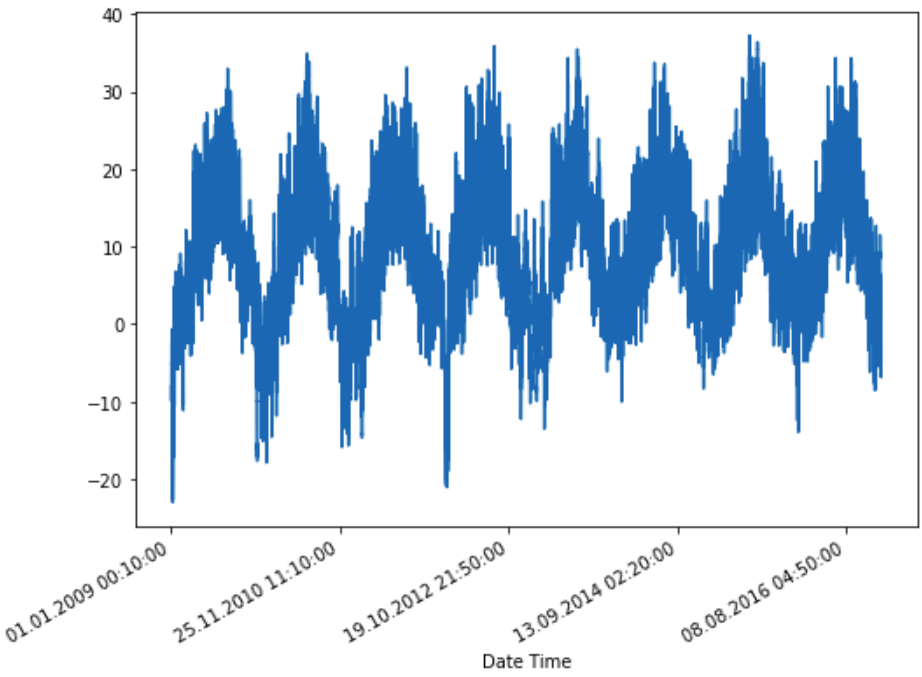
\includegraphics[scale=0.55]{1.png}
	\caption{Một phần của tập dữ liệu thu thập được}
\end{figure}


\leftskip0.0cm
\bigskip
\changefontsizes{14pt}
\setlength{\parindent}{0.5cm}
\textbf{1.2.2. Xử lý dữ liệu đầu.}

\smallskip
\changefontsizes{13pt}
\setlength{\parindent}{1cm}
\leftskip0.5cm
Trước hết, những tấm ảnh bị mờ, ảnh có độ phân giải thấp, ảnh có quá nhiều đối tượng cần nhận diện ở một khung hình nhỏ sẽ được loại bỏ khỏi tập dữ liệu.

Kế đến nhóm dùng công cụ hỗ trợ VGG Image Annotator, để đóng khung cho đối tượng trong ảnh và gắn label (label này cho biết sinh viên có đang mặc trang phục đúng quy định hay không.)
%fill here

\begin{figure}[h!]
	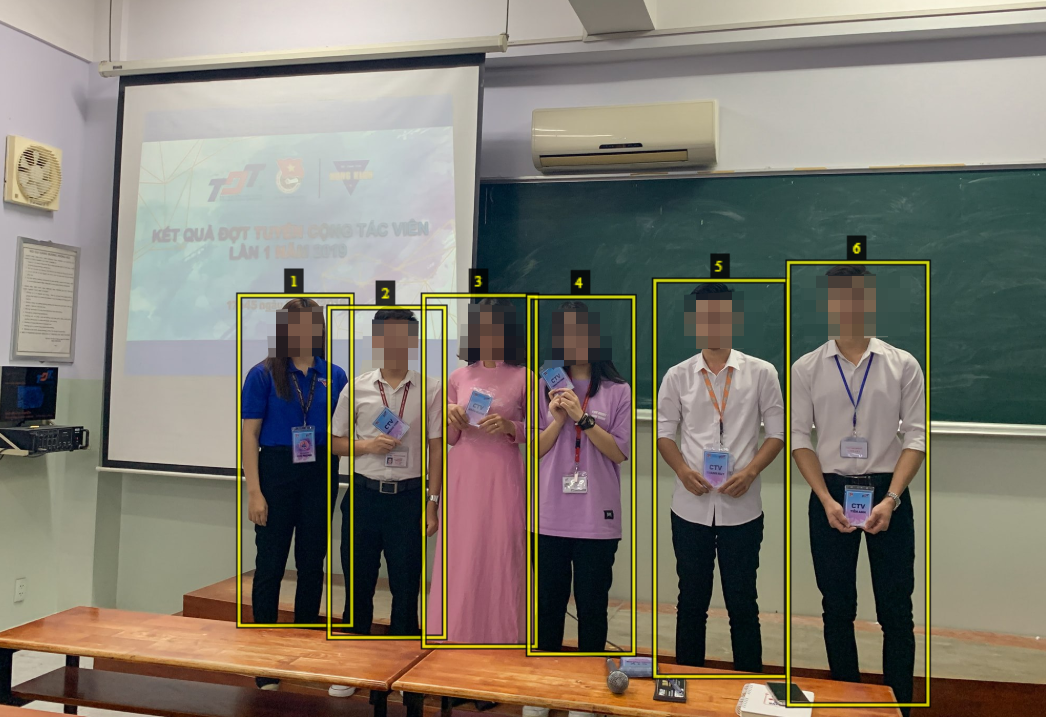
\includegraphics[scale=0.3]{2.png}
	\caption{Đóng khung và gắn label cho đối tượng}
\end{figure}

Sau khi đã đóng khung và gắn label cho toàn bộ ảnh trong tập (ngoại trừ một phần dữ liệu nhỏ dùng làm tập test cho model), từ công cụ trích xuất ra file .json lưu trữ thông tin về tên của ảnh và các tọa độ điểm cho từng khung trong từng ảnh. File .json và tập ảnh sẽ dùng để huấn luyện cho model của bài toán.

%Page ?? \clearpage

\leftskip0.0cm

\newpage
\changefontsizes{16pt}
\centerline{\textbf{\hyperlink{page.7}{CHƯƠNG 2: GIẢI THUẬT}}}



\bigskip
\changefontsizes{14pt}
\setlength{\parindent}{0.0cm}
\textbf{2.1. Thế nào là Object recognition và Classification?}

\smallskip
\changefontsizes{13pt}
\setlength{\parindent}{1cm}

%fill here
Về cơ bản, object recognition (hay object detection) là phương pháp nhận diện vị trí (tọa độ) của một đối tượng (object) trên một mặt phẳng (ở đây là ảnh). Classification là sự đánh giá (phân loại) đối tượng đó thuộc về lớp (label) nào. 

Với sự phát triển không ngừng của kỹ thuật và công nghệ, ngày nay có rất nhiều giải thuật dùng để nhận diện một đối tượng (Selective Search, DPM, R-CNN, Fast R-CNN, Faster R-CNN, Mask R-CNN, SSD, RetinaNet,...) và phân lớp đối tượng đó (KNN, Decision Tree, Naive Bayes, CNN,...).

Vì có những ưu và nhược điểm khác nhau, nên các giải thuật kể trên được sử dụng cho các trường hợp khác nhau. Và giải thuật phù hợp nhất theo đánh giá của nhóm cho đề tài này là YOLOv3 và CNN. 

\bigskip
\changefontsizes{14pt}
\setlength{\parindent}{0.0cm}
\textbf{2.2. YOLO.}


\smallskip
\changefontsizes{13pt}


%fill here
\setlength{\parindent}{1cm}
YOLO là viết tắt của từ You Only Look Once, đây sự nỗ lực đầu tiên trong việc xây dựng một thiết bị nhận diện vật thể (object detector) chạy với thời gian thực. Bởi vì YOLO chỉ \textit{Look Once} và không phải trải qua các bước trung gian như ở các giải thuật khác, nên tốc độ tính toán và cho ra kết quả của nó là cực kỳ nhanh.


\setlength{\parindent}{0.5cm}
\bigskip
\textbf{Luồng công việc (Workflow)}

\vspace{-0.35cm}
\begin{enumerate}
	\leftskip1cm
	\item Chuẩn bị trước một model CNN đã được train cho việc phân lớp
	\vspace{-0.25cm}
	\item Chia bức ảnh cần nhận diện và phân lớp đối tượng thành $S \times S$ ô (cell). Nếu có phần nào của một đối tượng nằm vào một ô, thì ô này là "tín nhiệm" cho việc phát hiện sự tồn tại của đối tượng đó. Tại mỗi ô, tính:
	
	\vspace{-0.35cm}
	 \begin{itemize}
	 	\leftskip1cm
	 	\item Tọa độ dự đoán của B khung (bounding boxes), trong $ B $ khung này có khả năng có một hoặc nhiều khung bao quanh được đúng đối tượng cần tìm.
	 	\vspace{-0.1cm}
	 	\item Độ tin cậy (confidence score), giá trị này thể hiện cho khả năng chứa một đối tượng của ô.
	 	\vspace{-0.1cm}
	 	\item $ K $ xác suất (probability), xác xuất tồn tại của đối tượng $C_i$ ($ i = 1,2,...K $) trong từng khung.
	 \end{itemize}
 	
 	\vspace{-0.5cm}
 	\item Tại lớp (layer) cuối của model CNN (đã chuẩn bị ở trên) điều chỉnh sao cho đầu ra (output) có dạng $ S \times S \times (5B + K) $. Bởi một ảnh có $ S \times S \times B$ khung, tại mỗi khung có 4 giá trị thể hiện cho tọa độ dự đoán, 1 cho độ tin cậy và K xác xuất tại mỗi ô.
\end{enumerate}

\begin{figure}[h!]
	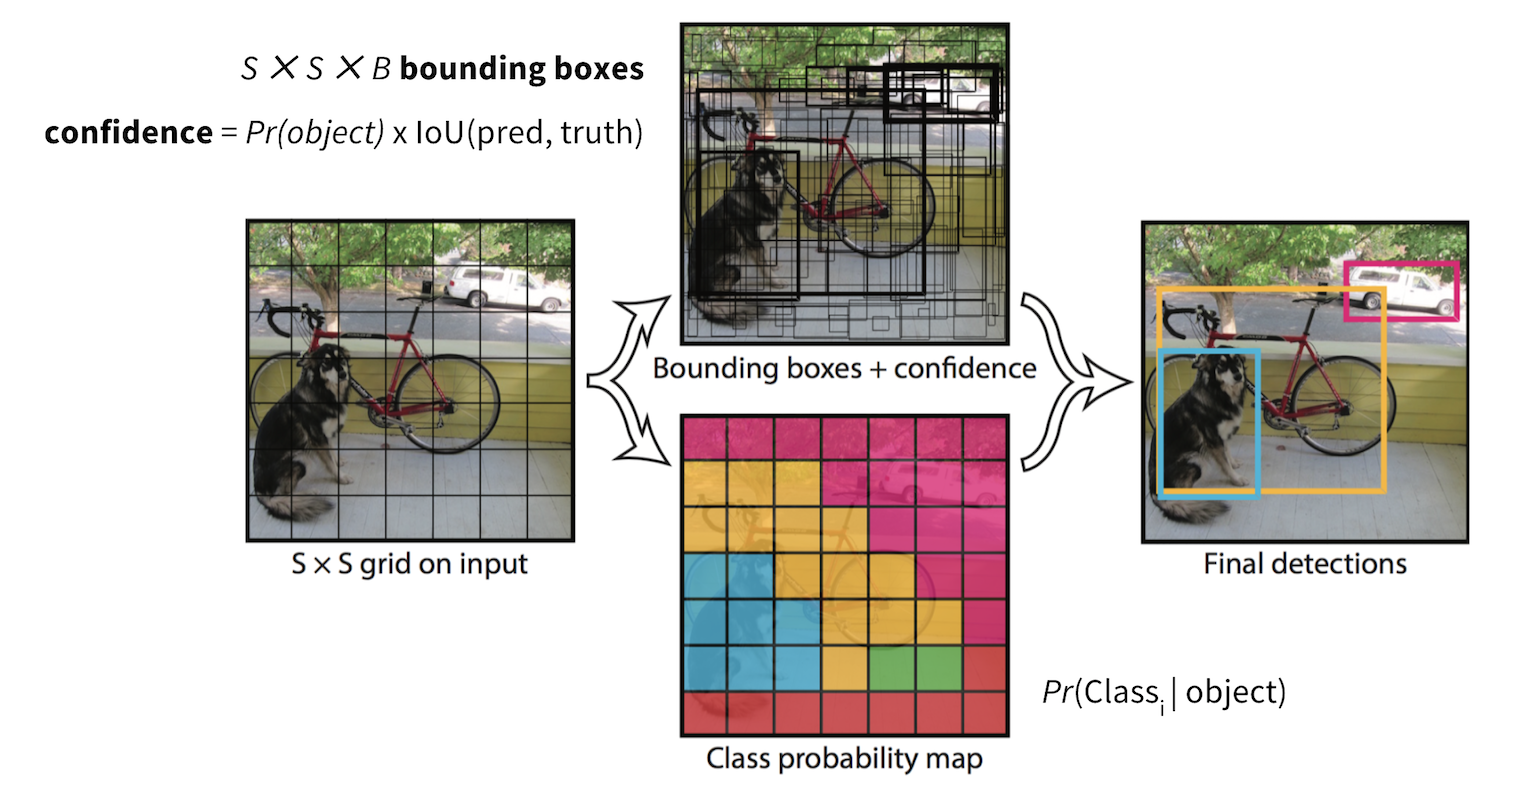
\includegraphics[scale=0.5]{yolo.png}
	\caption{Luồng công việc của model YOLO}
\end{figure}

\setlength{\parindent}{1cm}
Kết quả dự đoán cuối cùng có dạng $S \times S \times (5B + K) $ được tạo bởi hai lớp liên kết đầy đủ (fully connected layer) cho toàn bộ bản đồ đặc tính tích chập (convolutional feature map).


\begin{figure}[h!]
	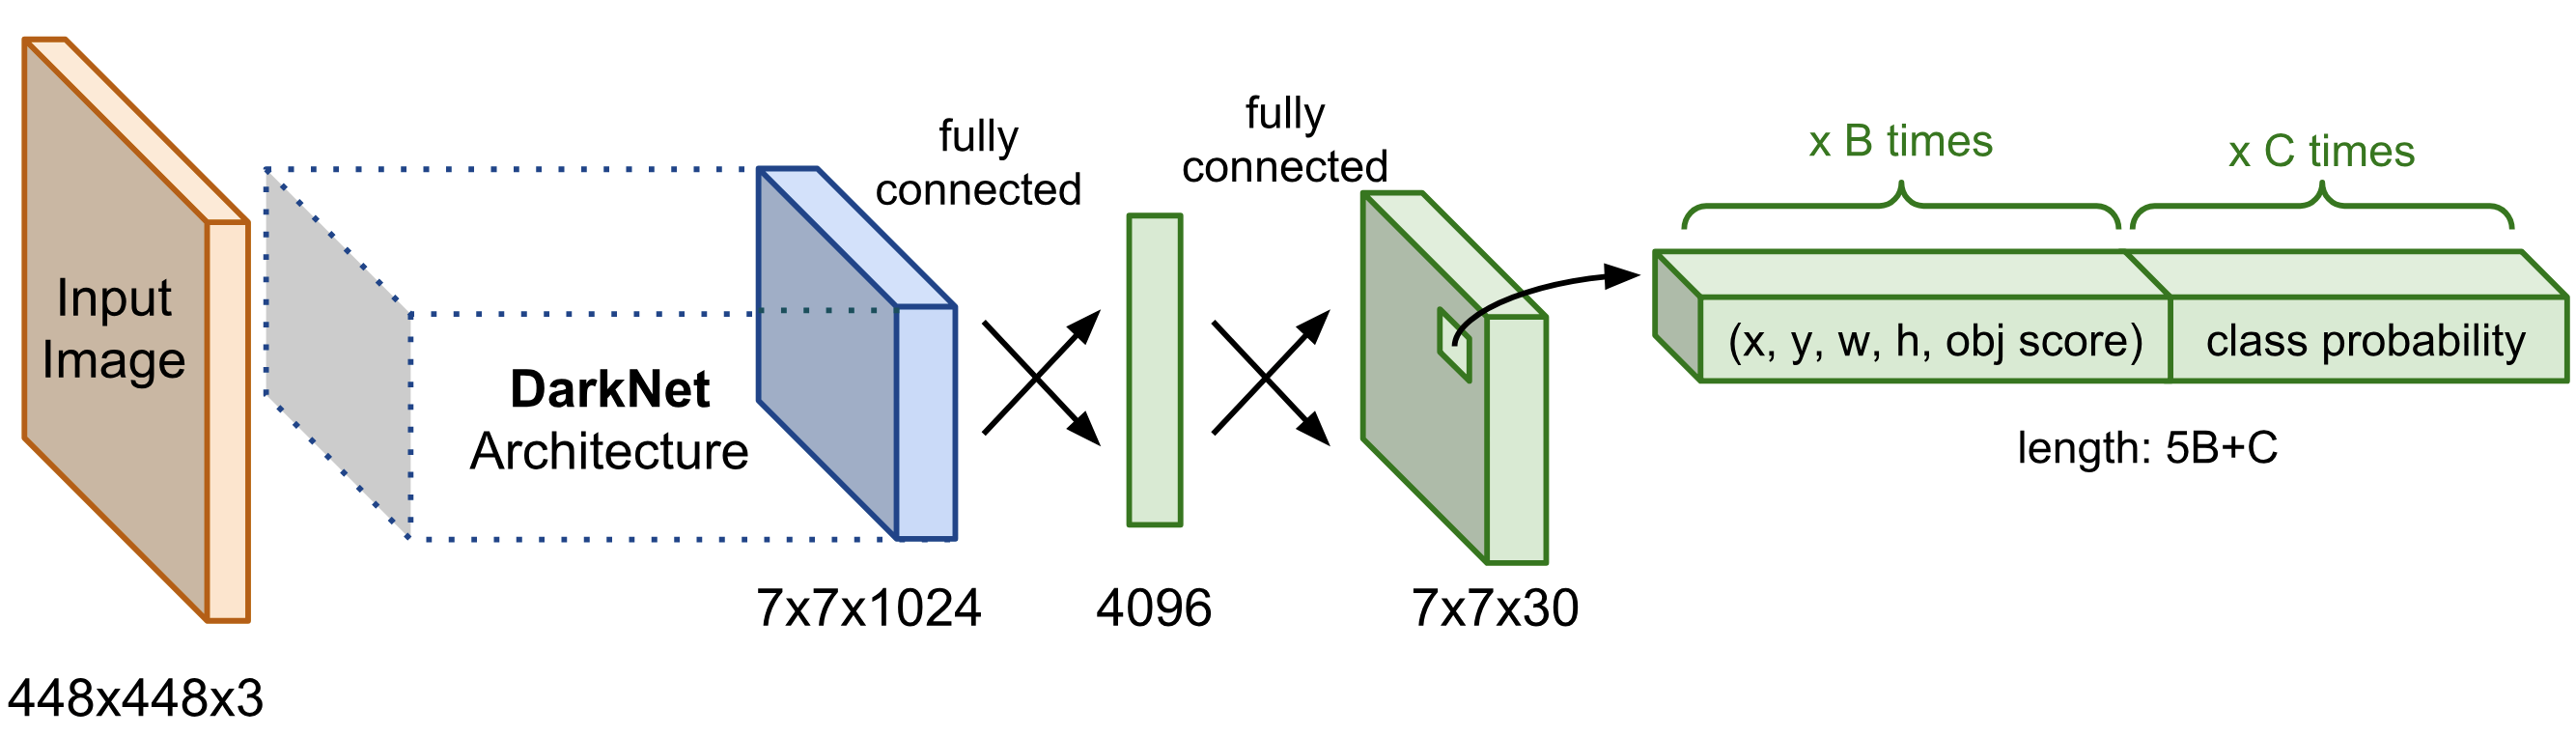
\includegraphics[scale=0.325]{yolona.png}
	\caption{Kiến trúc mạng (Network Architecture) của YOLO}
\end{figure}


\bigskip
\setlength{\parindent}{0.5cm}
\textbf{Mất mát (Loss Function)}


\leftskip0.5cm
\setlength{\parindent}{1cm}
\smallskip
Hàm tính mất mát dựa trên: tổng sai lệnh giá trị giữa dự đoán với thực tế của tọa độ khung (localization loss) và phân lớp (classification loss). Ngoài ra còn có hai tham số được dùng cho việc điều chỉnh các giá trị sai lệch (loss) mà chúng ta muốn xảy ra là $\lambda_\text{noobj}$ và $\lambda_\text{coord}$.


\leftskip0.0cm
$
\begin{aligned}
	\mathcal{L}_\text{loc} &= \lambda_\text{coord} \sum_{i=0}^{S^2} \sum_{j=0}^B {1}_{ij}^\text{obj} [(x_i - \hat{x}_i)^2 + (y_i - \hat{y}_i)^2 + (\sqrt{w_i} - \sqrt{\hat{w}_i})^2 + (\sqrt{h_i} - \sqrt{\hat{h}_i})^2 ] \\
	\mathcal{L}_\text{cls}  &= \sum_{i=0}^{S^2} \sum_{j=0}^B \big( {1}_{ij}^\text{obj} + \lambda_\text{noobj} (1 - {1}_{ij}^\text{obj})\big) (C_{ij} - \hat{C}_{ij})^2 + \sum_{i=0}^{S^2} \sum_{c \in \mathcal{C}} {1}_i^\text{obj} (p_i(c) - \hat{p}_i(c))^2\\
	\mathcal{L} &= \mathcal{L}_\text{loc} + \mathcal{L}_\text{cls}
\end{aligned} 
$


\leftskip0.5cm
\bigskip
Trong đó:
\begin{itemize}
	\leftskip1.5cm
	\item ${1}_i^\text{obj}$ Một hàm biểu thị liệu ô $i$ có chứa đối tượng nào hay không.
	\vspace{-0.2cm}
	\item ${1}_{ij}^\text{obj}$ Biểu thị khung thứ $j$ của ô $i$ có là khung tín nhiệm (xem hình 5) hay không.
	\vspace{-0.2cm}
	\item $C_{ij}$ Giá trị tin cậy của ô $i$.
	\vspace{-0.2cm}
	\item $\hat{C}_{ij}$ Giá trị tin cậy dự đoán của ô $i$.
	\vspace{-0.2cm}
	\item $\mathcal{C}$ Tập các lớp đối tượng có thể có.
	\vspace{-0.2cm}
	\item $p_i(c)$ Xác xuất chứa đối tượng $c$ của ô $i$, $c \in \mathcal{C}$.
	\vspace{-0.2cm}
	\item $\hat{p}_i(c)$ Xác xuất dự đoán đối tượng $c$ tồn tại trong ô $i$. 
\end{itemize}
\leftskip0.0cm

\smallskip
Trong hình 5, ta thấy có B khung (bounding box) nằm xung quanh ô (cell) $i$, trong đó có một khung (khung được in đậm) là có số vùng trùng khớp lớn nhất so với khung thực tế. Khung này được xem là khung dự đoán "tín nhiệm".

\begin{figure}[h!]
	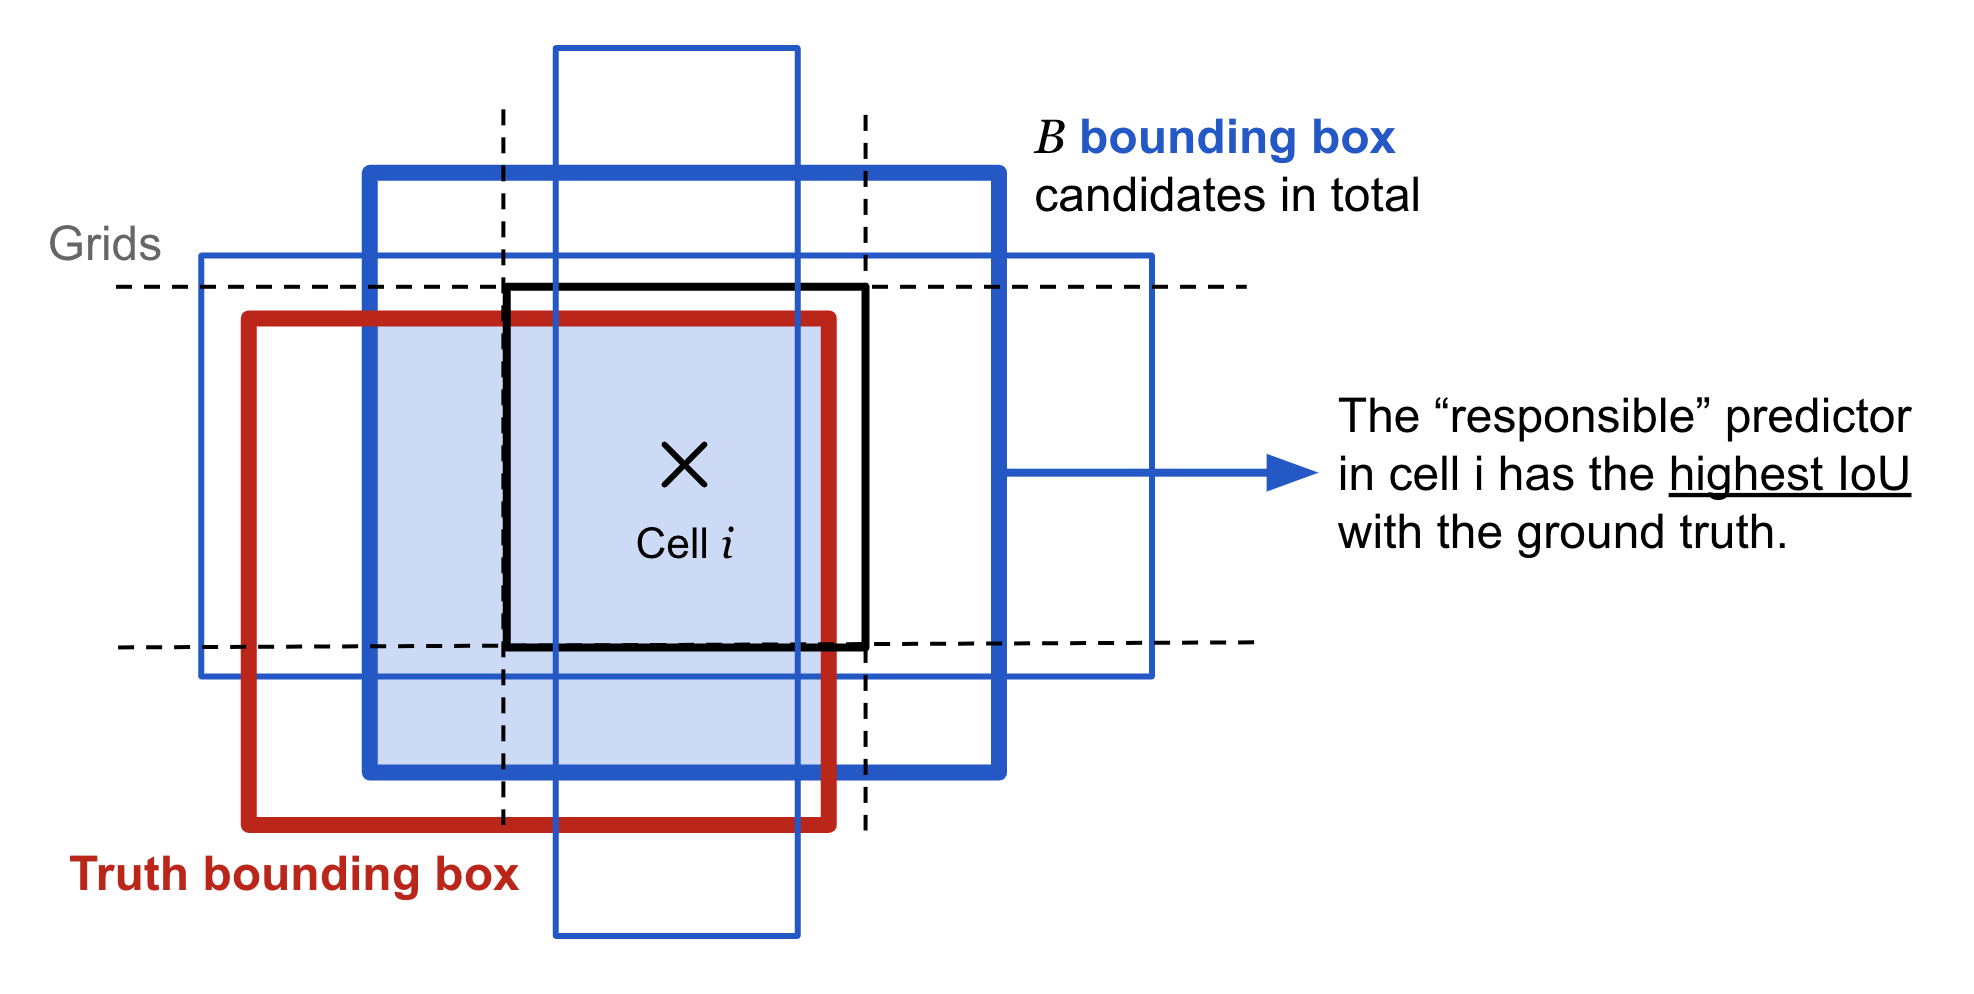
\includegraphics[scale=0.41]{yolobb.png}
	\caption{$B$ khung xung quanh ô $i$}
\end{figure}

\bigskip
\changefontsizes{14pt}
\setlength{\parindent}{0.0cm}
\textbf{2.3. YOLOv3.}

\smallskip
\changefontsizes{13pt}
\setlength{\parindent}{1cm}
YOLOv3 hay You Only Look Once version 3, đúng như cái tên đây là phiên bản cải tiến của YOLO thế hệ đầu. Danh sách các thay đổi gồm:

\vspace{-0.35cm}
\begin{enumerate}
	\leftskip1cm
	\item \textbf{Dùng hồi quy tuyến tính (Logistic regression) để tính độ tinh cậy}, trong khi YOLO phiên bản đầu tính dựa trên tổng bình phương các sai số.
	\vspace{-0.25cm}
	\item \textbf{Không còn sortmax}, YOLOv3 phân lớp bằng nhiều hàm logistic tuyến tính một cách độc lập (multiple independent logistic classifier).
	\vspace{-0.25cm}
	\item \textbf{Sử dụng Darknet + ResNet làm nền tảng}.
	\vspace{-0.25cm}
	\item \textbf{Dự đoán trên nhiều tỉ lệ hơn (Multi-scale prediction)}.
	\vspace{-0.25cm}
	\item \textbf{Bỏ qua lớp nối kết (concatenation layer)}.	
\end{enumerate}


%Page ??
\newpage
\changefontsizes{16pt}
\centerline{\textbf{\hyperlink{page.7}{CHƯƠNG 3: KẾT QUẢ}}}

%
\bigskip
\changefontsizes{14pt}
\setlength{\parindent}{0.0cm}
\textbf{3.1. Kết quả thực nghiệm.}

\smallskip
\changefontsizes{13pt}
\setlength{\parindent}{1cm}

%fill here
Nhóm đã quay video và tách ra thành từng frame làm dữ liệu test cho model sau khi đã huấn luyện. Dưới đây là một số output.


\begin{figure}[h!]
	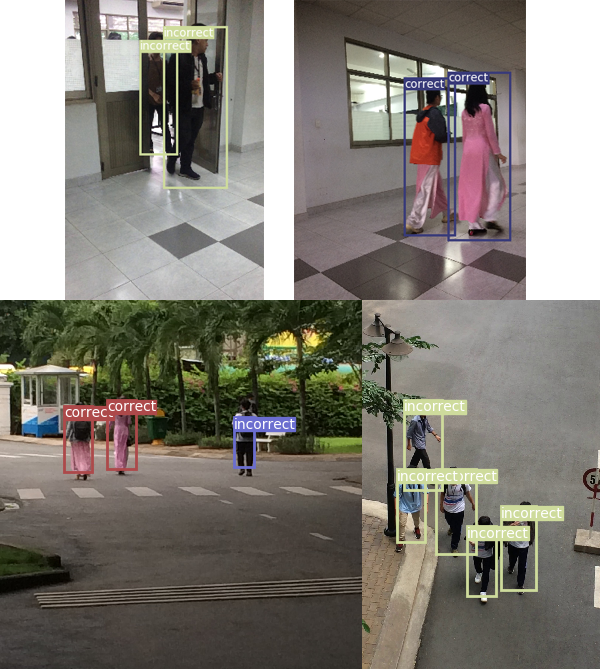
\includegraphics[scale=0.7]{test2.png}
	\caption{Kết quả thực nghiệm.}
\end{figure}




\bigskip
\changefontsizes{14pt}
\setlength{\parindent}{0.0cm}
\textbf{3.2. Đánh giá kết quả.}


\smallskip
\changefontsizes{13pt}
\setlength{\parindent}{1cm}

%fill here
Đã xác định được tối tượng và đánh giá được các trường hợp sinh viên mặc trang phục không đúng quy định.

Tuy nhiên do dữ liệu dùng để huấn luyện còn ít nên vẫn còn tồn tại một vài hạn chế.

Đầu tiên về phần xác định tọa độ của đối tượng trong ảnh vẫn còn sai số đáng kể, sai đối tượng.

Và với phần xác định trang phục có đúng quy định hay không, đôi khi hệ thống vẫn còn có sự nhầm lẫn giữa những trang phục có cùng màu sắc và đánh giá sai.

%Page ??
\newpage
\changefontsizes{16pt}
\centerline{\textbf{\hyperlink{page.7}{CHƯƠNG 4: TỔNG KẾT}}}


%
\bigskip
\changefontsizes{14pt}
\setlength{\parindent}{0.0cm}
\textbf{4.1 Thành quả đạt được.}

\smallskip
\changefontsizes{13pt}
\setlength{\parindent}{1cm}

%fill here
Nắm chắc các phương pháp trong môn Khai thác dữ liệu và khai phá tri thức, biết được cách thu thập và xử lý dữ liệu để có một model tốt. Các giải thuật đã được tìm hiểu rõ ràng hơn, đặc biệt là giải thuật về nhận diện và phân lớp đối tượng.

Khả năng phân công và hợp tác trong khi làm việc nhóm được cải thiện, công việc được hoàn thành hiệu quả và năng suất.

\bigskip
\setlength{\parindent}{0.0cm}
\changefontsizes{14pt}
\textbf{4.2. Hạn chế.}

\smallskip
\changefontsizes{13pt}
\setlength{\parindent}{1cm}

Dữ liệu thu thập còn ít, nên chưa tạo ra được sản phẩm đúng như mong đợi.

\bigskip
\setlength{\parindent}{0.0cm}
\changefontsizes{14pt}
\textbf{4.3. Hướng mở rộng.}

\smallskip
\changefontsizes{13pt}
\setlength{\parindent}{1cm}

Nếu hệ thống được huấn luyện với tập dữ liệu lớn sẽ có thể hoạt động chính xác và chi tiết hơn. Ví dụ sinh viên có đang đóng thùng hay không.

Kết hợp với camera an ninh của trường sẽ dễ dàng nhận diện được sinh viên ăn mặc không đúng quy định và xử phạt. Giúp nâng cao ý thức cho mỗi sinh viên, hình thành được tính kỷ luật giúp ít cho công việc sau này.

%fill here

%




%Page ?? + 1
\newpage
\changefontsizes{16pt}
\centerline{\textbf{\hyperlink{page.7}{TÀI LIỆU THAM KHẢO}}}

\vspace{1.2cm}
\changefontsizes{14pt}
\setlength{\parindent}{0cm}
\textbf{Tiếng Việt}

\bigskip
\changefontsizes{13pt}
\setlength{\parindent}{1cm}



[1]https://deepmlml.com › classic-object-detection

\vspace{3cm}
\changefontsizes{14pt}
\setlength{\parindent}{0cm}
\textbf{Tiếng Anh}


\bigskip
\changefontsizes{13pt}
\setlength{\parindent}{1cm}

[1]\url{https://pjreddie.com/darknet/yolo/}

[2]\url{https://lilianweng.github.io/lil-log}

\end{document}